% Backseat architecture diagram.
%
% Build:  tectonic docs/architecture.tex
%         pdftocairo -png -r 200 -transp -singlefile docs/architecture.pdf docs/architecture
%
% Two rules the layout follows, both learned the hard way.
%
% 1. HORIZONTAL. The pipeline is a left-to-right spine (capture, ring, grid,
%    tick, model, line) with exactly two satellites: the wakes above the tick,
%    which decide WHEN a tick happens, and the sound row below it, which is the
%    only part of the pipeline that never leaves the machine. A vertical version
%    of the same graph is a column that no README can show at a readable size.
%
% 2. TRANSPARENT PAGE, OPAQUE BOXES. The PNG is rendered with no background so
%    it sits on any page, which means every glyph has to survive both a white
%    and a dark backdrop. So all text lives INSIDE a filled box, and the only
%    ink outside a box is the arrows, drawn in a mid grey that reads either way.
%
% Routing: every edge is strictly orthogonal and no two edges touch. The sound
% row leaves the source box downward (`|-', vertical then horizontal) and enters
% the tick from below (`-|', horizontal then vertical), so it passes under the
% spine without ever crossing it.
\documentclass[border=12pt]{standalone}
\usepackage{tikz}
\usepackage[T1]{fontenc}
\usepackage{helvet}
\renewcommand{\familydefault}{\sfdefault}
\usetikzlibrary{arrows.meta, positioning}

% Small italic annotation, always inside a box (see rule 2 above).
\newcommand{\ann}{\scriptsize\itshape}

\begin{document}
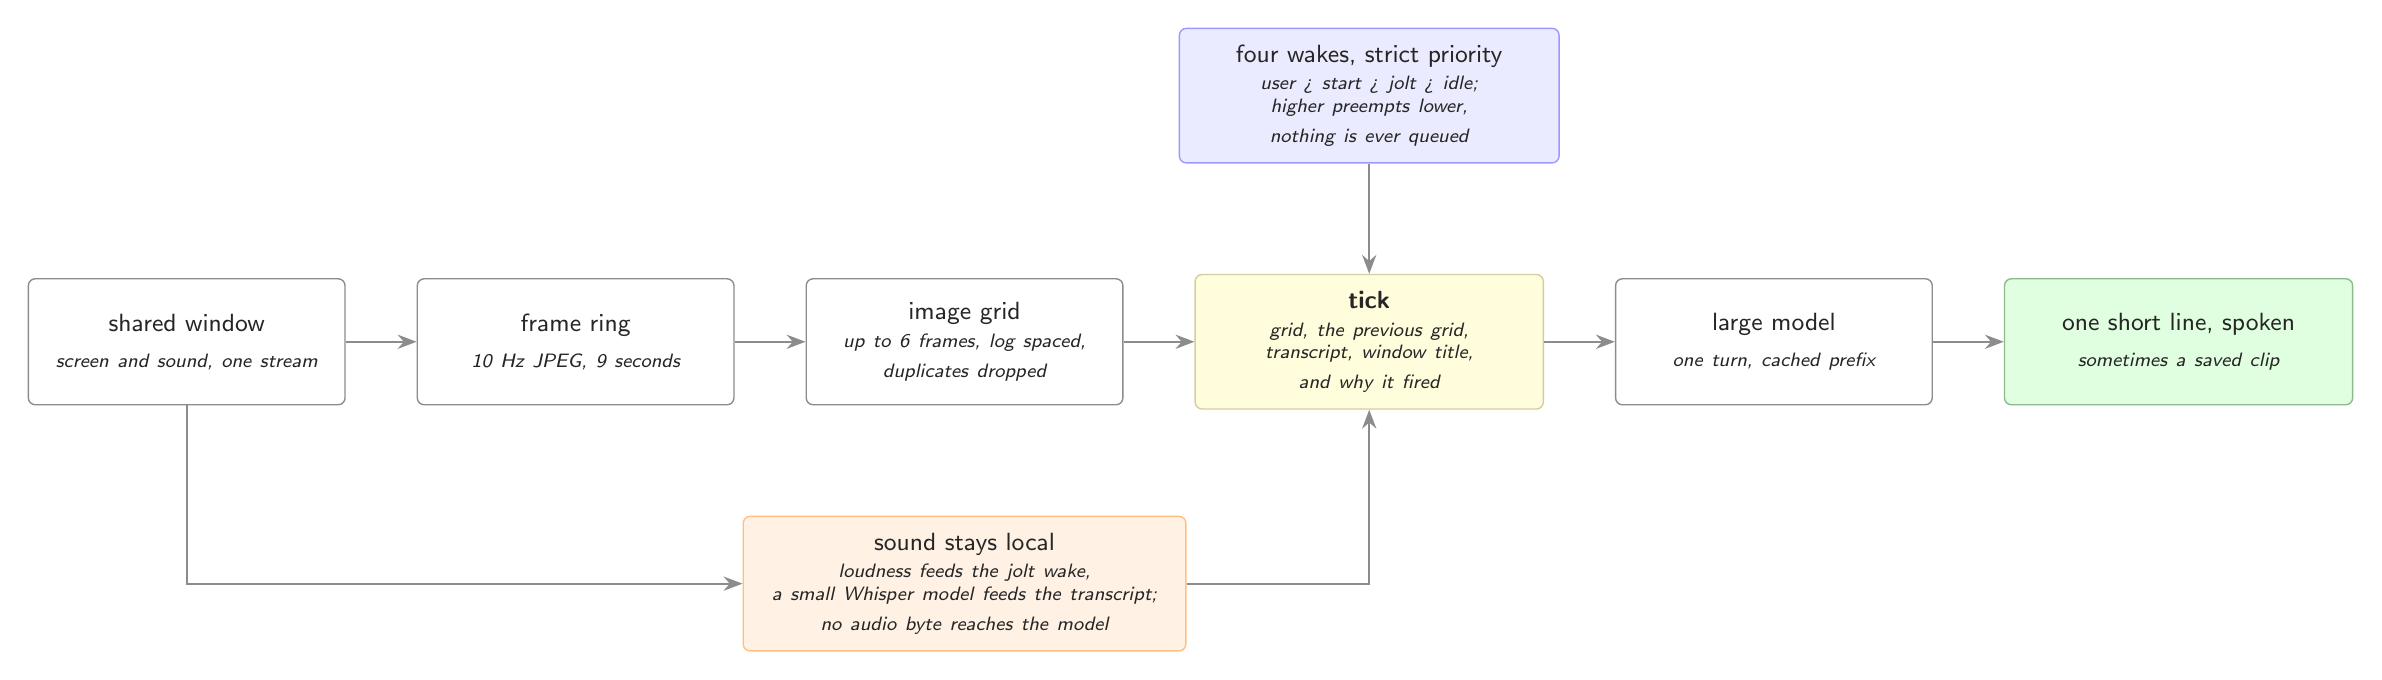
\begin{tikzpicture}[
  font=\small,
  node distance=9mm,
  box/.style={
    draw=black!45,
    fill=white,
    rounded corners=2.5pt,
    line width=0.5pt,
    align=center,
    inner sep=6pt,
    minimum height=16mm,
    text width=36mm,
    text=black!85,
  },
  wake/.style={box, fill=blue!8, draw=blue!40, text width=44mm},
  local/.style={box, fill=orange!10, draw=orange!50, text width=52mm},
  key/.style={box, fill=yellow!14, draw=yellow!55!black!45, text width=40mm},
  result/.style={box, fill=green!12, draw=green!40!black!45, text width=40mm},
  flow/.style={draw=black!45, line width=0.8pt, -{Stealth[length=2.4mm]}},
]

% ---- the spine, left to right ---------------------------------------------
\node[box] (src)
  {shared window\\[2pt]
   {\ann screen and sound, one stream}};
\node[box, right=of src] (ring)
  {frame ring\\[2pt]
   {\ann 10 Hz JPEG, 9 seconds}};
\node[box, right=of ring] (grid)
  {image grid\\[2pt]
   {\ann up to 6 frames, log spaced,\\ duplicates dropped}};
\node[key, right=of grid] (tick)
  {\textbf{tick}\\[2pt]
   {\ann grid, the previous grid,\\ transcript, window title,\\ and why it fired}};
\node[box, right=of tick] (llm)
  {large model\\[2pt]
   {\ann one turn, cached prefix}};
\node[result, right=of llm] (reply)
  {one short line, spoken\\[2pt]
   {\ann sometimes a saved clip}};

\draw[flow] (src)  -- (ring);
\draw[flow] (ring) -- (grid);
\draw[flow] (grid) -- (tick);
\draw[flow] (tick) -- (llm);
\draw[flow] (llm)  -- (reply);

% ---- what decides WHEN, above the tick ------------------------------------
\node[wake, above=14mm of tick] (wakes)
  {four wakes, strict priority\\[2pt]
   {\ann user > start > jolt > idle;\\ higher preempts lower,\\ nothing is ever queued}};
\draw[flow] (wakes) -- (tick);

% ---- what never leaves the machine, below the spine -----------------------
% Placed under the grid so both of its edges run along a clear row: down from
% the source on the left, up into the tick on the right.
\node[local, below=14mm of grid] (audio)
  {sound stays local\\[2pt]
   {\ann loudness feeds the jolt wake,\\ a small Whisper model feeds the transcript;\\ no audio byte reaches the model}};
\draw[flow] (src.south) |- (audio.west);
\draw[flow] (audio.east) -| (tick.south);

\end{tikzpicture}
\end{document}
